\documentclass[a4paper]{article}

\usepackage{INTERSPEECH2016}

\usepackage{graphicx}
\usepackage{amssymb,amsmath,bm}
\usepackage{textcomp}
\usepackage{verbatim}
\usepackage{cite}
\usepackage{upgreek}
\usepackage{url}

\def\vec#1{\ensuremath{\bm{{#1}}}}
\def\mat#1{\vec{#1}}


\sloppy % better line breaks
\ninept

\title{Entropy-based segmentation of birdcalls using Fourier transform phase}

%%%%%%%%%%%%%%%%%%%%%%%%%%%%%%%%%%%%%%%%%%%%%%%%%%%%%%%%%%%%%%%%%%%%%%%%%%
%% If multiple authors, uncomment and edit the lines shown below.       %%
%% Note that each line must be emphasized {\em } by itself.             %%
%% (by Stephen Martucci, author of spconf.sty).                         %%
%%%%%%%%%%%%%%%%%%%%%%%%%%%%%%%%%%%%%%%%%%%%%%%%%%%%%%%%%%%%%%%%%%%%%%%%%%
%\makeatletter
%\def\name#1{\gdef\@name{#1\\}}
%\makeatother
%\name{{\em Firstname1 Lastname1, Firstname2 Lastname2, Firstname3 Lastname3,}\\
%      {\em Firstname4 Lastname4, Firstname5 Lastname5, Firstname6 Lastname6,
%      Firstname7 Lastname7}}
%%%%%%%%%%%%%%% End of required multiple authors changes %%%%%%%%%%%%%%%%%

\makeatletter
\def\name#1{\gdef\@name{#1\\}}
\makeatother \name{{\em Author Name$^1$, Co-author Name$^2$}}

\address{$^1$Author Affiliation \\
  $^2$Co-author Affiliation \\
  {\small \tt author@university.edu, coauthor@company.com}
}

%\twoauthors{Karen Sp\"{a}rck Jones.}{Department of Speech and Hearing \\
%  Brittania University, Ambridge, Voiceland \\
%  {\small \tt Karen@sh.brittania.edu} }
%  {Rose Tyler}{Department of Linguistics \\
%  University of Speechcity, Speechland \\
%  {\small \tt RTyler@ling.speech.edu} }

%
\begin{document}

  \maketitle
  %
  \begin{abstract}
  In this  paper we describe an entropy-based algorithm for the segmentation of
  birdcalls from recordings. The entropy of time-frequency blocks are estimated
  from the phase of the Fourier transform. To overcome difficulties in
  processing the phase, the group delay function from an all-pole filter is
  utilised. The group delay function has good frequency resolution properties,
  and hence provides reliable estimates of the entropy. Furthermore, spectral
  whitening is performed to smooth the entropy estimate and the extremities are
  determined. A threshold is applied on the difference to distinguish the call
  periods from the background.  The algorithm is evaluated on two different
  datasets, one of which is recorded in more challenging field conditions. When
  compared to entropy estimated from the power spectrum, the entropy from the
  group delay function provides better detection accuracy at almost all
  operating points. The choice of model order of the all-pole filter for
  different bird species is also briefly investigated.
  \end{abstract}
  \noindent{\bf Index Terms}: bioacoustics, birdcall segmentation, Fourier transform phase
  



\section{Introduction}

With the advent of automated recording devices (for eg. the SongMeter series from Wildlife
Acoustics Inc. \cite{sm3}), the collection of large amounts of
bioacoustic data has become relatively easy. By analysing birdcalls collected in
this manner, it is possible to perform tasks such as the tracking of migrant
species or examining the avian biodiversity of a given region. Typically, the
collected data is processed offline. In this process, the first step is usually to
determine regions of interest in the recording (also called segmentation.) An 
entropy-based bird phrase segmentation
technique was developed in \cite{wang2013}. In this paper, we propose a modified
version of that technique, by using information from the phase of the short-term
Fourier transform (STFT). Most techniques for processing speech and audio signals have
utilised the magnitude spectrum of the STFT. Although the phase spectrum of the STFT has 
useful information, its processing has remained difficult. A popular technique
for exploiting information from the phase has been through group delay functions. In
this work, we utilise information from group delay functions using parametric
models, and apply it to segment birdcalls into active and inactive regions.

The group delay function has good frequency resolution properties, which enable
it to be useful in tasks such as speech recognition and speaker recognition
\cite{hema} \cite{padman} \cite{modgdf}. The same property is beneficial in the
processing of bird vocalizations. In \cite{wang2013}, the entropy within a
sliding time-frequency window over the spectrogram has been effectively used for
distinguishing active and inactive regions. The essential idea is that birdcalls
have more structure (for eg.~harmonics may be present), and thus have lower
entropy when compared to background sounds, which have higher entropy. This
difference in entropy levels enable effective distinction between birdcalls and
the background.
%Applying a similar technique with the group delay function, rather than the
%spectrogram, provides increased frequency resolution, and hence more effective
%entropy computation. 
The high resolution property of group delay functions enable accurate tracking
of time-frequency information. In this work, the entropy of a sliding
time-frequency window is estimated from the group delay representation. Spectral
whitening is applied to smooth the entropy estimates and thresholding on
differences of extrema is performed to separate the birdcalls from the
background.

Many studies on birdcalls have used manual segmentation \cite{Trifa} \cite{Lee}
\cite{Kaewtip}. Time domain segmentation using energy has been used in many
studies \cite{Harma} \cite{Somervuo} \cite{Fagerlund} . The energy  based
segmentation method is highly influenced by background noise and will
deteriorate  where bird calls have low energy in comparison to the background. A
KL-divergence based segmentation method is proposed in \cite{Lakshmi}.
KL-divergence between normalized power spectral density of a frame and uniform
distribution is computed. The more KL-divergence corresponds to less entropy and
vice-versa. Local minima of KL-divergence act as change points for bird
vocalizations. In \cite{Neal}, time-frequency based segmentation using a random
forest classifier is proposed to  segment the bird vocalizations from a noisy
audio recording. 

\section{Utilising Fourier transform phase}

Commonly used features for processing speech and audio signals are based on the
magnitude spectrum of the short-term Fourier transform. The phase spectrum has
received relatively lesser attention due to signal processing difficulties, one
of them being the need to unwrap the phase spectrum. The unwrapping problem can
be bypassed by utilising the group delay function, which is the negative
derivative of the phase spectrum. The group delay function can be computed using
properties of the Fourier transform, and hence avoids the need for explicit
computation of the phase spectrum. The group delay function
$\uptau(\omega)$ can be derived as \cite{gdDeriv}
\begin{equation}
\uptau(\omega) = \frac{X_R(\omega) Y_R(\omega) + X_I(\omega)
Y_I(\omega)}{|X(\omega)|^2},
\label{eq:gdelayFormula}
\end{equation}
where $x(n) \leftrightarrow X(\omega)$ and $y(n) \leftrightarrow Y(\omega)$ are
Fourier transform pairs and $y(n) = n x(n)$.  However, $\uptau(\omega)$, as
computed above can produce artifacts in the form of spurious peaks at spectral
nulls. These nulls correspond to zeros close to the unit circle when the vocal
tract transfer function is represented in the $Z$ domain.  At spectral nulls,
the value of the denominator in equation \ref{eq:gdelayFormula} tends to zero,
leading to spurious peaks which mask the formant structure
\cite{hema},\cite{hemaSigProc1989},\cite{chirpGD}.  Several methods have been
proposed in the literature to overcome the effects due to these artifacts
\cite{modgdf}, \cite{productSpectrum}, \cite{chirpGD}. Another technique to
overcome this difficulty is to model the vocal tract as an all-pole filter,
hence avoiding the zeros altogether. Such a technique derived using linear
prediction (LP) analysis was used in the detection of formants in human speech
\cite{yegnaFormant}. 

The vocal tract is represented in the LP model as
\begin{equation}
H(\omega) = \frac{G}{1-\sum_{k=1}^{P} a(k) e^{-j \omega k}},
\label{eq:lpModel}
\end{equation}
where the predictor model order is $P$, $G$ represents the gain and $a(k)$ are
the predictor coefficients\cite{makhoul}.
The filter reprsented by $H(\omega)$ is an all-pole filter, and its group delay
function does not suffer from the artifacts mentioned earlier. The all-pole 
group delay function (APGDF) is defined as
\begin{equation}
\uptau_A(\omega) = \frac{X_R(\omega) Y_R(\omega) + X_I(\omega)
Y_I(\omega)}{|H(\omega)|^2},
\label{eq:apGdelayFormula}
\end{equation}
which is obtained by replacing the power spectrum in the denominator of equation
\ref{eq:gdelayFormula} with the all-pole power spectrum of equation
\ref{eq:lpModel}. This avoids spectral nulls in the denominator of equation
\ref{eq:apGdelayFormula}, thus retaining the formant structure in the group
delay function.

Figure \ref{fig:all-pole} shows the magnitude spectrum, LP
spectrum and APGDF derived from a 20 ms call of Cassins vireo (\textit{Vireo
cassinii.}) As can be seen, the APGDF emphasises the formants, as compared to the
DFT magnitude spectrum or the LP magnitude spectrum. Two peaks which are merged
in the magnitude spectra around the 100th frequency bin appear distinctly in the
APGDF.

\begin{figure}[h]

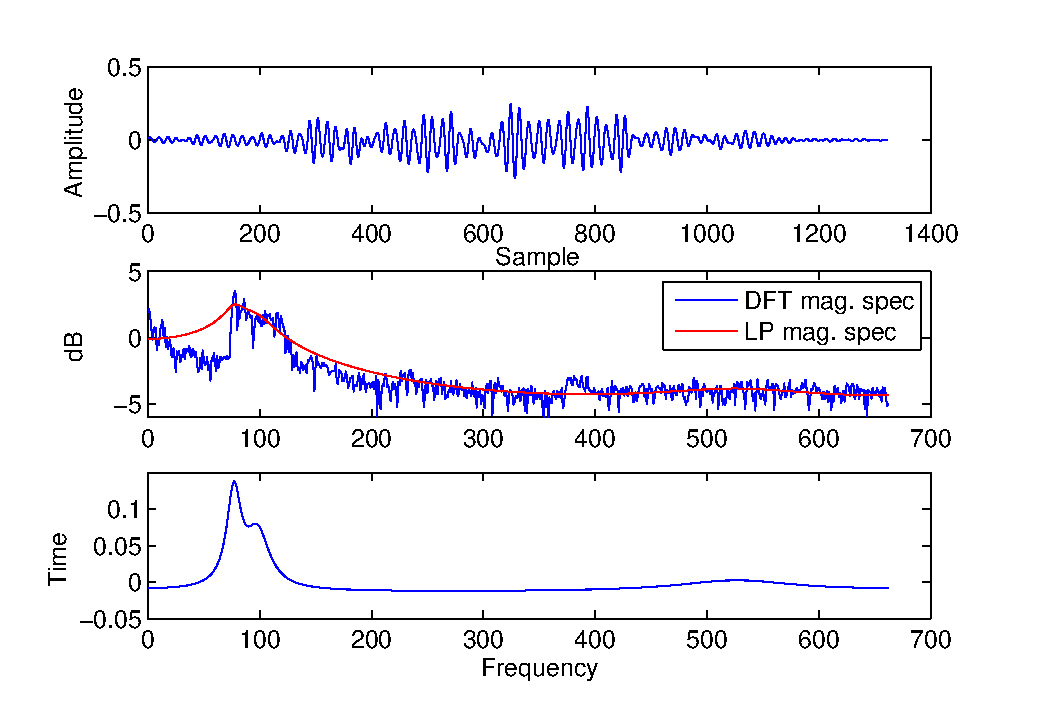
\includegraphics[width=0.5\textwidth,height=7cm]
{apgd.eps}
\caption{ A frame of audio signal (top panel), corresponding LP
magnitude spectrum superimposed on DFT magnitude spectrum (middle panel) and
all-pole group delay function (bottom panel)  }
\label{fig:all-pole}
\end{figure}


Recently, feature vectors
derived from such a representation were used in speech \cite{drugman} and speaker
recognition \cite{padman}. 


There is strong evidence that birds use their vocal tract as a selective filter
to modify the final sound \cite{catchpole}.  Given this, the source-filter model
developed for analysing human speech can be applied to bird vocalizations as
well.  LP analysis of human speech signals models the vocal
tract spectrum as an all-pole filter \cite{makhoul} excited by a single source.
When applied to birdcalls, this is a simplification of the `two-voice' theory of
avian vocalization\cite{catchpole}, in that there is assumed to be only one
source, rather than two. Nevertheless, this reasonable assumption is followed in
this work. A similar assumption has been made in \cite{agnihotri}, where LP
analysis has been applied in analysing the song of the greater racket-tailed
drongo.


%This is equivalent to a cascade of several
%first-order and second-order all-pole filters. The overall magnitude spectrum is
%the product of the individual magnitude spectra, and the overall phase spectrum
%is the sum of the individual phase spectra \cite{yegnaFormant}. Although
%developed for human speech, th

\section{Entropy-based segmentation of birdsong}

Computing the APGDF for every frame enables good time-frequency resolution of
the audio recording. Unlike the power spectrum, the APGDF can be negative.
Since here we are interested only in the magnitudes and locations of the
frequency components, the sign of the APGDF is ignored by taking the absolute
value. Henceforth, APGDF means positive APGDF.  A sliding time-frequency window
of width $w$ frames and frequency range $f_{\min}$ to $f_{\max}$ is considered over the
APGDF vectors. As in \cite{wang2013}, the entropy of this window is estimated
using the expression
\begin{equation}
\label{eq:2}
 h_{k}=-\sum_{n=kT+1}^{kT+w}\sum_{f=f_{\min}}^{f_{\max}} \uptau_N(n,f) \ln \uptau_N(n,f),
\end{equation}
where $T$ is the time-frequency window shift and $\uptau_N(n,f)$ is normalized
APGDF. $\uptau_N(n,f)$ is estimated using the expression 
\begin{equation}
\label{eq:3}
\uptau_N(n,f)=\frac {\uptau_A(n,f)}
{\sum_{n=kT+1}^{kT+w}\sum_{f=fmin}^{fmax} \uptau_A(n,f)},
\end{equation}
where $\uptau_A(n,f)$ is the APGDF at frame $n$ and frequency $f$.

The entropy calculated from the time-frequency window is less susceptible to sudden
changes in the background as compared to the entropy calculated at each time
instance \cite{wang2013}. The entropy of the time-frequency window containing
birdcalls is lower than the one only containing the background. As the
window moves to the call region from the background, there is a gradual drop in
entropy. 
%The entropy remains low if time-frequency window completely
%overlaps with the call period. The entropy increases as the window moves from
%call region to background. 

%The APGDF from figure
%\ref{fig:apgd} is shown in \ref{fig:apgdNoSign} after ignoring the sign.
%\begin{figure}[h]
%\centering
%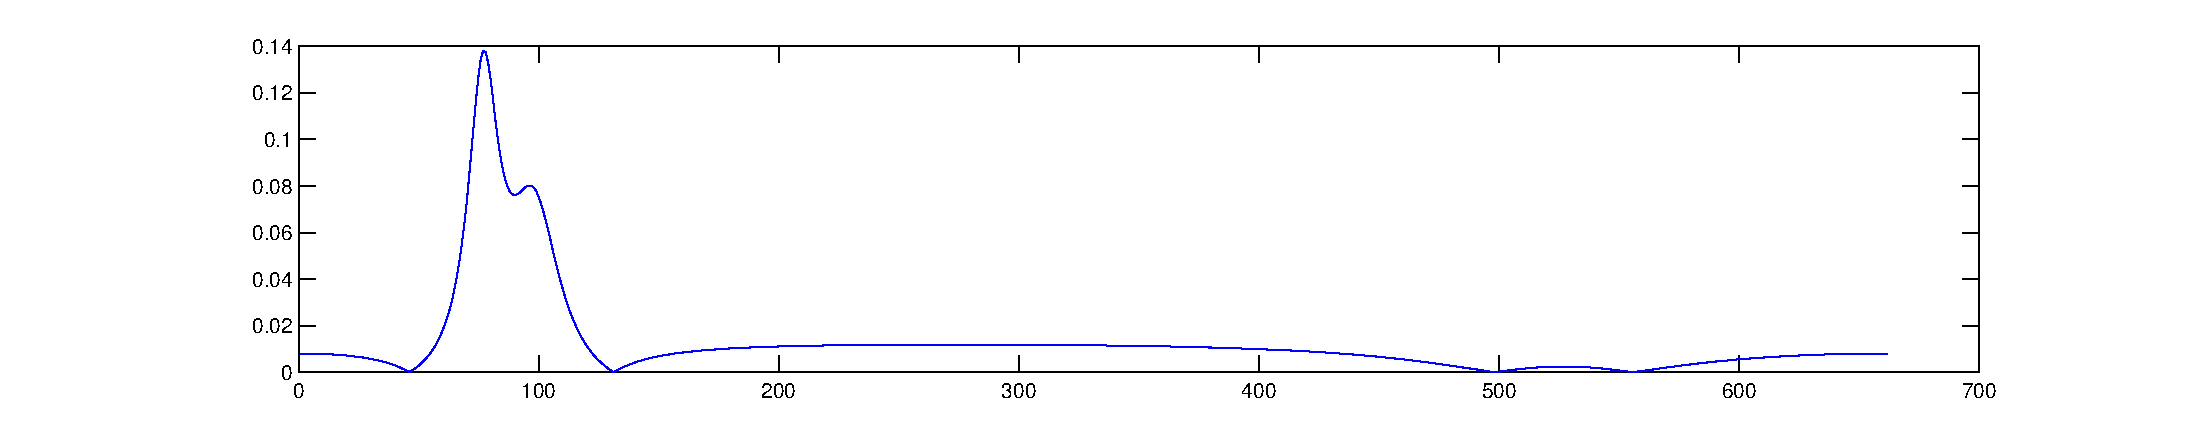
\includegraphics[width=0.5\textwidth,height=2cm]{apgdNoSign.eps}
%\caption{based on all pole model (in the bottom panel).}
%\label{fig:all-pole}
%\end{figure}



 


\subsection{Whitening the APGDF before entropy calculation}

The drop in entropy during the presence of bird vocalizations makes it possible
to detect call periods. Due to the presence of various background sounds e.g.
rain, thunder, other animals etc., entropy of the background can  vary rapidly
making it difficult to separate it from the entropy during a call period. To
mitigate this problem to some extent, as in \cite{wang2013}, the APGDF is
whitened before calculating the entropy. The entropy calculated from the
whitened APGDF is almost constant for the background but dips enough to mark the
presence of bird vocalizations. Due to this, small changes in entropy can be
detected fairly reliably. 
%Therefore, the whitened APGDF is used to calculate the
%entropy.

To whiten the APGDF ($\uptau_A$), the covariance matrix $C$ of the mean-subtracted
APGDF is estimated. The eigenvalue matrix $S$ and the eigenvector matrix
$U$ of $C$ are determined. The whitened APGDF
($\uptau_W$) is calculated as
\begin{equation}
\label{eq:4}
\uptau_W=\text{diag} \bigg(  \frac{1}{\sqrt{\text{diag($S$)}+\epsilon}} 
\bigg )\times \text{$U^T$} \times \uptau_A
\end{equation}

Here $\epsilon$ is a negligible positive number added to prevent division by zero. 
 The difference
between entropy calculated from the original APGDF and the whitened APGDF is
evident in figure \ref{fig:entropy}.

\begin{figure}[h]
\centering
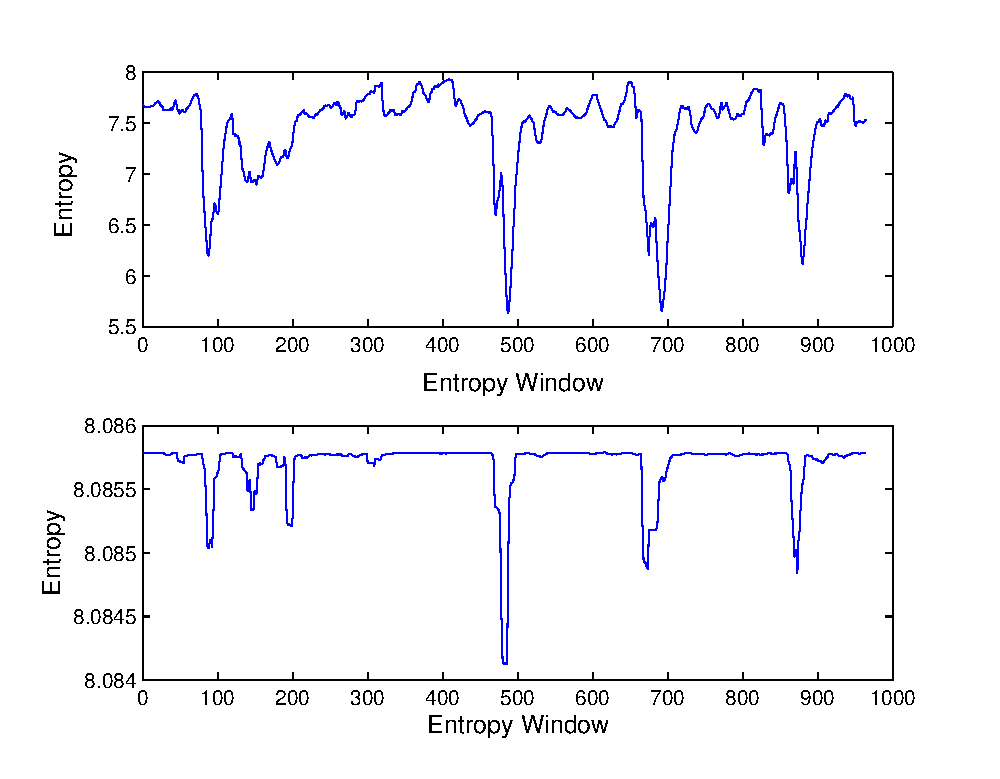
\includegraphics[width=0.5\textwidth,height=7.5cm]{Entropy_gd_white_non_white.eps}
\caption{ Entropy calculated from APGDF (Uppen Panel) and entropy calculated using white APGDF (Lower Panel).}
\label{fig:entropy}
\end{figure}



\subsection{Detecting change points using thresholding}
To detect change points, extrema-based thresholding is used. Local minima and
maxima are estimated on the entropy, and a threshold is applied on the
difference between consecutive minima and maxima. Two contiguous change points
correspond to the start and end of a bird vocalization. These change points can
be tracked back to get the start and end time of the vocalization in the
recording.     
   
\section{Performance analysis}


The proposed algorithm is evaluated on two datasets. The first consists of
recordings of a single species, the Cassin's vireo; the second consists of
recordings from several species, and is a subset of the MLSP 2013 bird
classification challenge.
In the Cassin's vireo dataset \cite{data1}, the total duration
of recordings is about 45 minutes, out of which about 5 minutes correspond to
the calls. These recordings are collected over two months and are fairly clean.
Phrase annotations are provided with the dataset, the start and end of which
are used as the ground truth for segmentation. 

The MLSP 2013 dataset \cite{data2} is much nosier and includes wind and rain in
the background. The recordings are done for over two years at 13 different
locations. Twenty five files of ten seconds length each are selected from this
data to evaluate the proposed method.  Manual annotations are done to mark the
presence of bird vocalizations in these audio files. The audio files contain
about 60 bird vocalizations, which occupy 13.35\% of the total time of
recordings.

The proposed algorithm is compared with a modified version of technique proposed
in \cite{wang2013}. Entropy estimated from the whitened power spectrum is used
to determine the change points. Similar to the proposed algorithm, extrema-based
thresholding is used to determine the change points. Thus, in the experiments,
entropy estimated from the power spectrum is compared to the entropy estimated
from the APGDF.
 
A frame length of 20 ms and increment of 5 ms is used to perform short-time
processing. APGDF computed on each frame is whitened before computing the
entropy as given in equation \ref{eq:4}. A time-frequency window of length $w$=138.8 ms
is used along with a shift of $T$ = 15 ms to estimate the entropy (see
equation \ref{eq:2}). The frequency range of the
time-frequency window is set from $f_{\min}$=1.5 kHz to $f_{\max}$=7 kHz
\cite{wang2013}. Although these parameters are possibly species specific, 
we use the same parameters for both datasets.

Receiver operating characteristics (ROC) curves are used to analyze the
performance of both techniques. True positive rate (TPR) and false alarm rate
(FAR) are calculated as:

\begin{equation}
\text{TPR} (\%)=\frac{\text{Correctly Classified Call Frames}}
{\text{Total Call Frames}} \times 100 
\end{equation}

\begin{equation}
\text{FAR} (\%)=\frac{\text{Wrongly Classified Call Frames}}
{\text{Total Background Frames}} \times 100 
\end{equation}

Figures \ref{fig:ROCdata1} and  \ref{fig:ROCdata2} depict ROC curves comparing
performance of the two methods on the respective datasets. It is clear from
figures \ref{fig:ROCdata1} and  \ref{fig:ROCdata2} that the APGDF-based
technique outperforms the power spectrum based method at most of the  operating
points.

\begin{figure}[h]
\centering
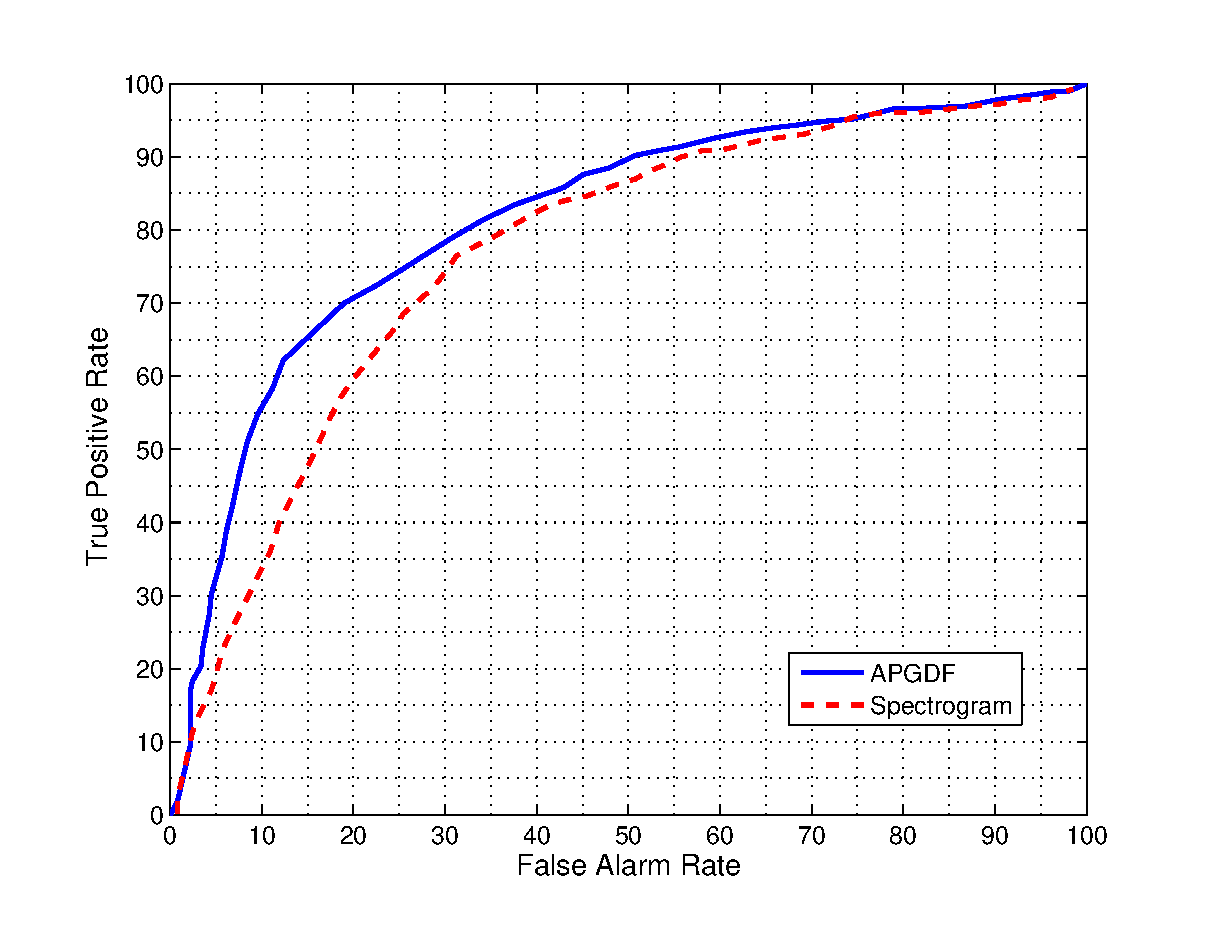
\includegraphics[width=0.5\textwidth,height=7cm]{gd1.eps}
\caption{ROC  curves  comparing  performance  of  methods based on APGDF and 
spectrogram on Cassin's Vireo dataset.}
\label{fig:ROCdata1}
\end{figure}
 
\begin{figure}[!ht]
	\centering
	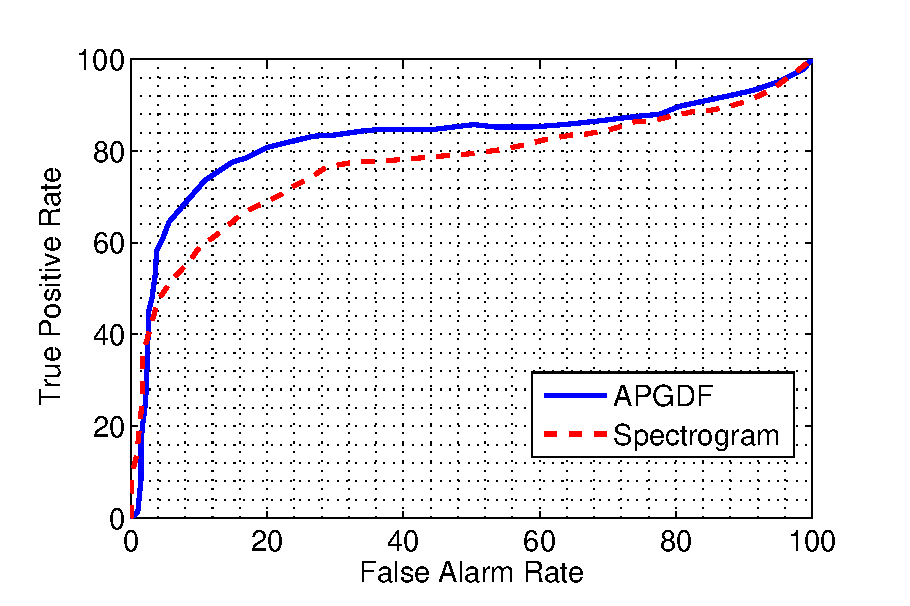
\includegraphics[width=0.5\textwidth,height=7cm] {gd2.eps}
	\caption{ROC curves comparing performance of methods based on APGDF and 
	spectrogram on MLSP dataset.}   
	\label{fig:ROCdata2}
\end{figure} 

It is to be noted that the method in \cite{wang2013} utilises a sophisticated
Bayesian change-point detection technique. When compared to the simple
thresholding technique used in our evaluation, their method acheives a better
true positive rate at 20\% false alarm rate (see figure 2 in \cite{wang2013}).
Replacing thresholding with a more relaiable change-point detection technique 
is expected to bring improvements while using the APGDF-based technique.

\subsection{Determining the model order for LP analysis}

To correctly model the all-pole filter while estimating the APGDF, one requires
to know the optimum number of poles to be used. In \cite{makhoul}, the Akaike
information criterion (AIC) is used to determine the optimal model order for the
LP filter. Assuming a Gaussian probability distribution for the signal, the
criterion approximated as
\begin{equation}
I(p) = \log V_p + 
\end{equation}
where $V_p$ is
XXX fill this up, and mention what is $N_e$.

For the Cassin's vireo, the AIC is computed for various model orders. The AIC
curve reaches a minimum around $p$=10 and then increases with a gentle slope. In
practice, a model order between 5 and 10 is well suited for this species.
To investigate if this is species specific, a similar study is performed for
four species from four different families. These are: Indian nightjar
(\textit{Caprimulgus asiaticus asiaticus} from the family Caprimulgidae, emerald
dove (\textit{Chalcophaps indica}) from the family Columbidae, abd XXX XXX.
The model order versus AIC plots given in figure XXX also indicate that the same value
of $p$ (between 5 and 10) is suitable accross multiple species.

 \begin{figure}[!ht]
	\centering
	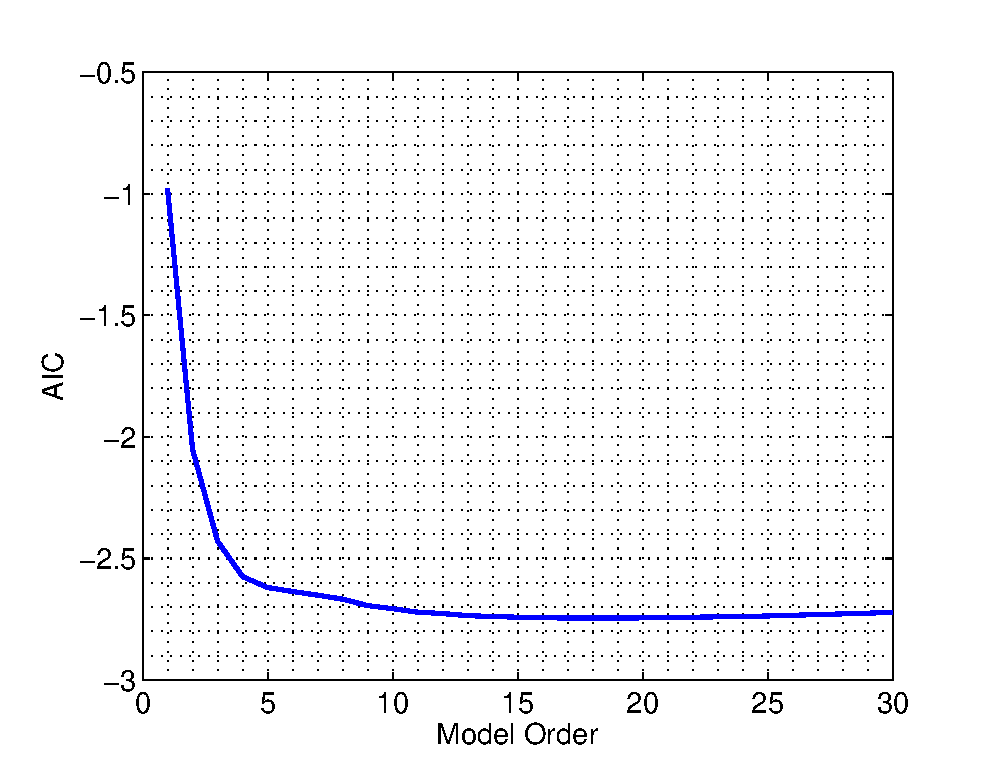
\includegraphics[width=0.5\textwidth,height=7cm] {cassins_AIC.eps}
	\caption{AIC vs model order for Cassin's Vireo }   
	\label{fig:AIC_cassins}
\end{figure} 

 
 
%Figure \ref{fig:AIC_3} depicts the AIC for different model orders for three
%different bird species i.e. Cuckoo, Great Barbet and Laughing Thresh. 
%
% \begin{figure}[!ht]
%	\centering
%	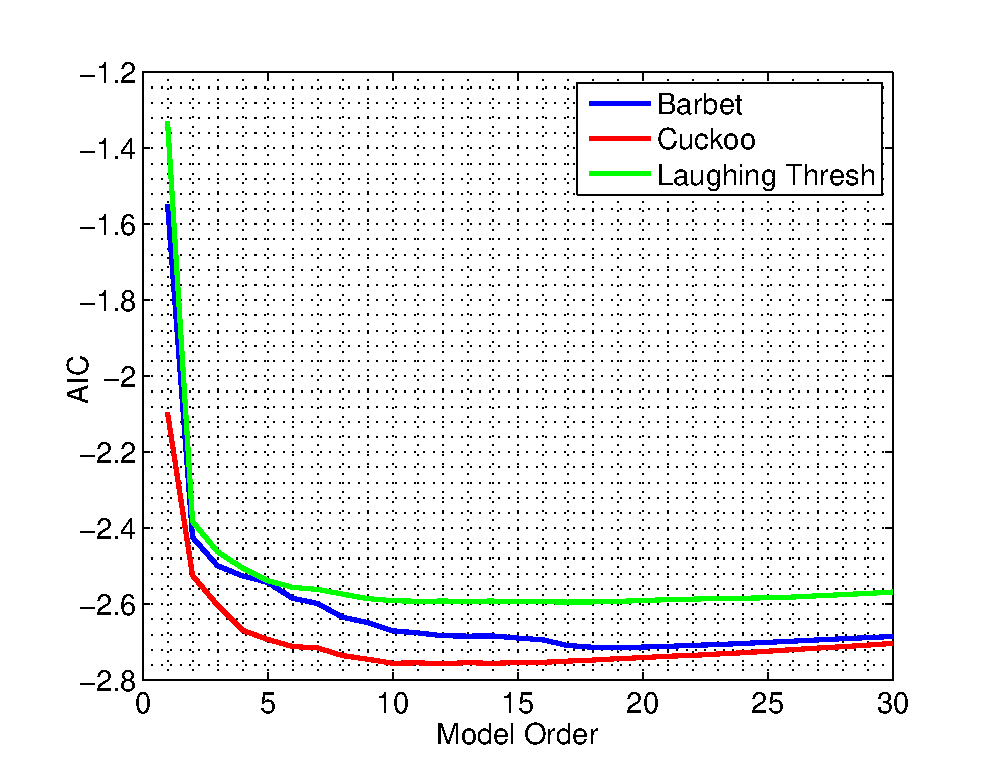
\includegraphics[width=0.5\textwidth,height=7 cm] {model_order_vs_AIC.eps}
%	\caption{AIC vs model order for three different species }   
%	\label{fig:AIC_3}
%\end{figure} 


 Figure \ref{fig:species_4} depicts the AIC for different model orders for four
 different bird species i.e. Indian Nightjar, Emerald Dove, Canary Flycatcher
 and Sarus Crane . 
 
 
 \begin{figure}[!ht]
	\centering
	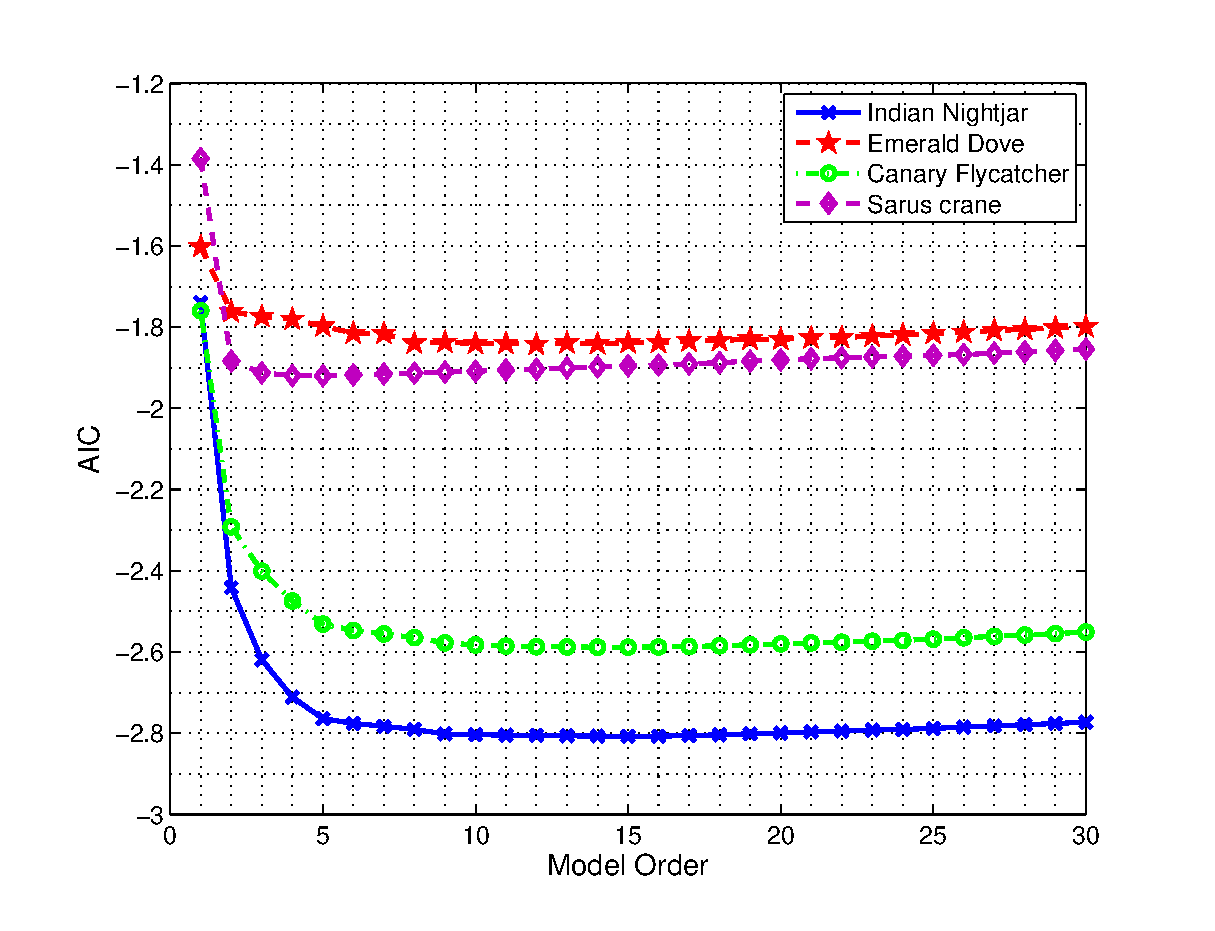
\includegraphics[width=0.5\textwidth,height=7 cm] {species_4.eps}
	\caption{AIC vs model order for four different species }   
	\label{fig:species_4}
\end{figure} 
 
 
 
 
% Figures \ref{fig:gd1_3} and \ref{fig:gd2_3} compare the performance of new and old APGDF.
% \begin{figure}[!ht]
%	\centering
%	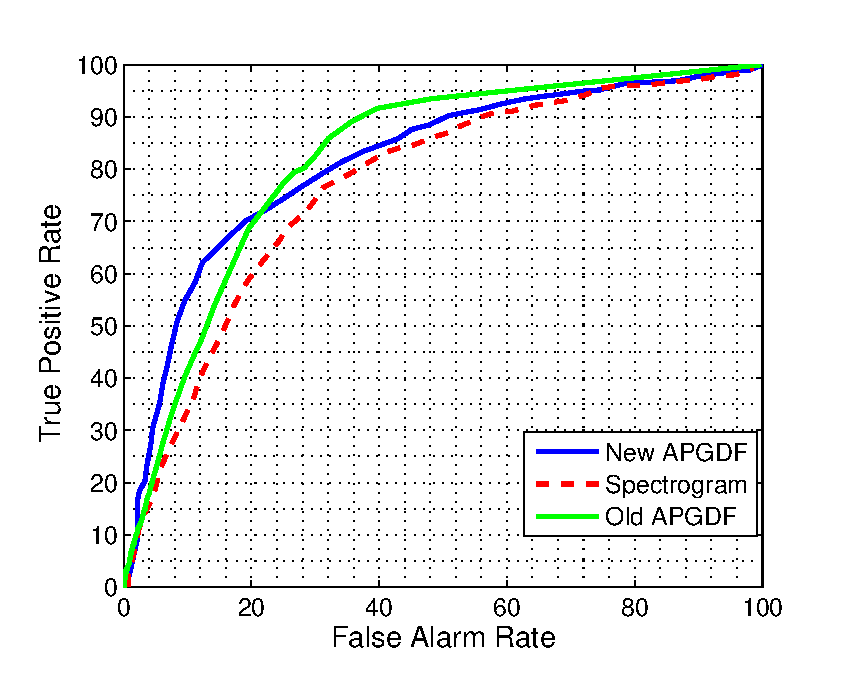
\includegraphics[width=0.5\textwidth,height=7 cm] {gd1_3.eps}
%	\caption{ROC curves comparing performance of methods based on old APGDF, new APGDF and spectrogram on Cassin's Vireo dataset }   
%	\label{fig:gd1_3}
%\end{figure} 
%
% 
% 
% \begin{figure}[!ht]
%	\centering
%	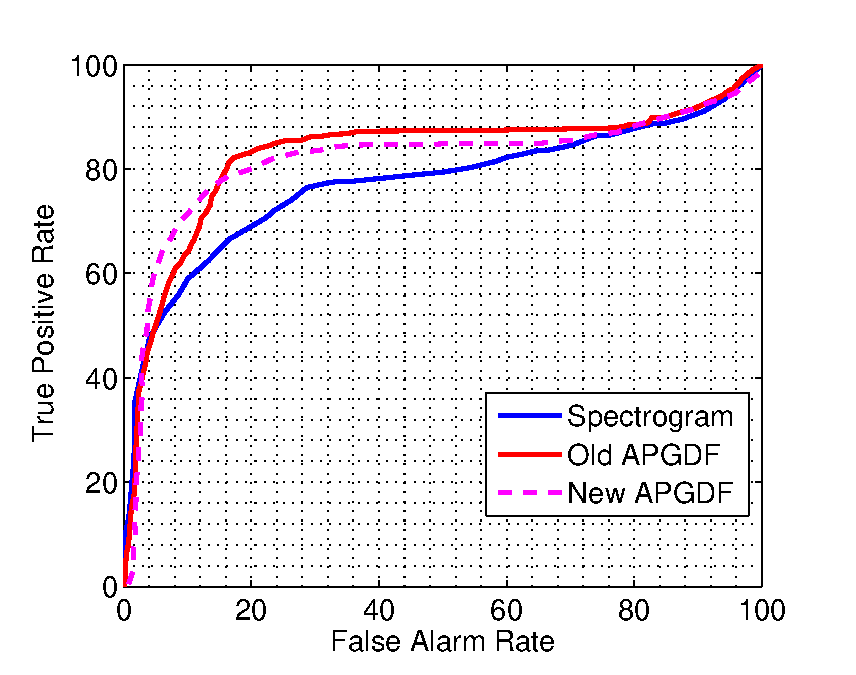
\includegraphics[width=0.5\textwidth,height=7 cm] {gd2_3.eps}
%	\caption{ROC curves comparing performance of methods based on old APGDF, new APGDF and spectrogram on MLSP dataset }   
%	\label{fig:gd2_3}
%\end{figure} 
 
 
 
 



 
\section{Conclusion}
In this paper, we explored an entropy-based birdcall segmentation technique. The
method utilises information from the phase spectrum of the short term Fourier
transform. To avoid the difficulty of unwrapping the phase, the group delay
function is utilised. An all-pole filter using LP analysis is used to model the
vocal tract spectrum while estimating the group delay function, resulting in the
APGDF represntation. The APGDF is whitened before estimating the entropy, and
extrema-based thresholding is performed to distinguish call periods from the
background. When compared to the entropy estimated from the power spectrum, the
entropy from the APGDF resulted in better segmentation accuracy.

Studies on model order for the LP filter using the Akaike information criteria
showed that a value of $p$ between 5 and 10 is sufficient for species from
different families. Future work will include applying the LP model to perform
tasks such as phrase detection and species identification.

  \newpage
  \eightpt
  \bibliographystyle{IEEEtran}

  \bibliography{mybib}

\end{document}
